\documentclass{beamer}
\usetheme{CambridgeUS}
\usecolortheme{beaver}
\usepackage{xeCJK}
\usepackage{hyperref}
\usefonttheme[onlymath]{serif}
\begin{document}

\begin{frame}
    \title{砸题选讲}
    \author{不保证题目按照难度递增排列}
    \begin{titlepage}
    \end{titlepage}
\end{frame}

\begin{frame}{CF102512D Equality}
    \begin{itemize}
        \item 有两个人,第一个人会在$[a_1, b_1], [a_2, b_2], \cdots, [a_X, b_X]$这些时间段在线
        \item 第二个人会在$[c_1, d_1], [c_2, d_2], \cdots, [c_Y, d_Y]$这些时间段在线
        \item 你需要统计有多少个$T$,满足在$1\sim N$的时间内的$T, 3T, 5T,\cdots$时刻第一个人在线,
        $2T, 4T, 6T, \cdots$时刻第二个人在线
        \item $N \leq 10^9, X, Y\leq 300$
    \end{itemize}
\end{frame}

\begin{frame}{CF102512D Equality}
    \begin{itemize}
        \item 对于一个确定的$T$,如何快速判断是否合法
        \item 我们将每个人的在线时间翻转,求出其不在线的时间
        \item 条件等价于对于第一个人,不存在时刻$(2k + 1)T$使得这个时刻被包含在某个不在线的区间内
        \item 对于第二个人,不存在时刻$2kT$使得这个时刻被包含在某个不在线的区间内
        \item 于是我们得到了一个$O(X + Y)$检查一个$T$是否合法的做法
    \end{itemize}
\end{frame}

\begin{frame}{CF102512D Equality}
    \begin{itemize}
        \item 考虑将所有的$T$按照是否小于等于$\sqrt N$分为两类
        \item 对于小于$\sqrt N$的部分直接暴力,时间复杂度$O(\sqrt N(X + Y))$
        \item 对于大于$\sqrt N$的部分,注意到$\frac{N}{T} \leq \sqrt N$
        \item 考虑第一个人的一段不在线时间$[l, r]$会导致哪些$T$不合法,即存在一个$k$使得
        $l \leq (2k + 1)T \leq r \Rightarrow \lceil\frac{l}{2k + 1}\rceil \leq T \leq \lfloor\frac{r}{2k + 1}\rfloor$
        \item 当$T \geq \sqrt N$的时候$k$非常小,因此可以枚举所有的$k$
        \item 时间复杂度$O(\sqrt N(X + Y))$
    \end{itemize}
\end{frame}

\begin{frame}{CF1286D LCC}
    \begin{itemize}
        \item 有一个对撞机,对撞机里面有一些质子,第$i$个质子的位置在$x_i$,速度为$v_i$
        \item 在实验开始的时候,每个质子会随机一个方向(左或者右)发射出去,第$i$个质子朝右发射的概率是$p_i$
        \item 问实验开始后期望多久会发生第一次碰撞,如果实验结束之前都没有发生任何碰撞,则认为碰撞时间为$0$
        \item $n \leq 10^5, v \leq 10^6, x \leq 10^9$,对$998244353$取模
    \end{itemize}
\end{frame}

\begin{frame}{CF1286D LCC}
    \begin{itemize}
        \item 容易发现第一次碰撞一定是两个最开始相邻的质子撞在一起,因此我们只需要考虑相邻两个质子的碰撞事件
        \item 将问题转化为求出碰撞时间$\geq k$的概率
        \item 对每个位置位置维护一个$2\times 2$的矩阵代表$dp$。即$dp[i][j]$表示考虑前$i$个质子,
        所有碰撞事件的发生时刻都大于$k$,最后一个质子朝向$j$的概率
        \item 对于一个限制$k$,相当于我们ban掉了某些位置的某些转移,那么将对应矩阵的这个转移的系数置为$0$即可
        \item 线段树维护矩阵,需要支持单点修改、全局查询
    \end{itemize}
\end{frame}

\begin{frame}{CF1225G To Make 1}
    \begin{itemize}
        \item 定义函数$f(x)$,当$k \mid x$时$f(x) = f(\frac xk)$,否则$f(x) = x$
        \item 黑板上有$n$个数,每次你可以选择其中的两个数$a_1, a_2$,从黑板上擦去这两个数,然后写下$f(a_1 + a_2)$
        \item 问最终黑板上能否仅剩下$1$这一个数
        \item $n \leq 16, k, \sum a_i \leq 2000$,保证所有$a_i$都不能被$k$整除
        \item 要求构造方案
    \end{itemize}
\end{frame}

\begin{frame}{提示}
    \begin{itemize}
        \item 如果存在一个非负整数序列$\{b_i\}$,使得$1=\sum a_i k^{-b_i}$,那么原问题有解
        \item 否则一定无解
    \end{itemize}
\end{frame}

\begin{frame}{CF1225G To Make 1}
    \begin{itemize}
        \item 假如我们找到了一个满足这个条件的序列,如何构造答案呢
        \item 令$B=\max b_i$,将这个式子两边同时乘以$k^B$
        $$\begin{aligned}
            k^B = \sum a_i k^{B - b_i}
        \end{aligned}$$
        \item 这个式子的每一项均是整数,考虑它们对$k$的整除性
        \item 等式左边显然可以被$k$整除,右边对于$B\neq b_i$的每一项,它们也能被$k$整除
        \item 这意味着,$\sum\limits_{b_i = B} a_i$可以被$k$整除
        \item 而给出的$a_i$保证了每个$a_i$均不被$k$整除,故至少存在两个$b_i = B$
    \end{itemize}
\end{frame}

\begin{frame}{CF1225G To Make 1}
    \begin{itemize}
        \item 假设这两个取到最大值的位置分别为$i,j$
        \item 将黑板上$a_i, a_j$这两个数擦去,写下$f(a_i + a_j)$
        \item 同时更新$b_i$,这时我们认为$j$这个位置已经不存在了
        \item 容易发现得到的这些数仍然没有一个数能被$k$整除,因此我们可以不断重复这个找最大值的过程,直到只剩下一个数
        \item 在整个过程中等式始终成立,因此最后得到的数一定是$1$
    \end{itemize}
\end{frame}

\begin{frame}{CF1225G To Make 1}
    \begin{itemize}
        \item 那么我们只需要找到这样一个序列$b$就可以了
        \item 设$dp[s][j]$表示已经考虑了$s$集合中的数,是否存在一个序列$b$使得$\sum\limits_{i \in s}a_ik^{-b_i} = j$
        \item 转移有两种:在当前集合中加入一个数,并将其$b_i$设为$0$;将当前集合中的所有$b_i$都减去$1$
        \item 可以通过$dp$值倒推出序列$b$
        \item 需要使用bitset优化,复杂度$O(\frac{2^n\sum a_i}{w})$
    \end{itemize}
\end{frame}

\begin{frame}{ZJOI2019 开关}
    \begin{itemize}
        \item 有$n$个开关,一开始所有开关都是关上的
        \item 给定一个状态$s$,你要使得第$i$个开关到达状态$s_i$
        \item 每个开关都有一个权值$p_i$,每一轮会选择一个开关,翻转这个开关的状态。第$i$个开关被选择的概率是$\frac{p_i}{\sum p_j}$
        \item 问期望多少轮之后所有开关均达到目标状态
        \item $n\leq 100, \sum p_i\leq 2000$
    \end{itemize}
\end{frame}

\begin{frame}{ZJOI2019 开关}
    \begin{itemize}
        \item 令$P = \sum p_i$,然后让每个$p$都除以$P$
        \item 枚举最后每个开关被操作了多少次,由于最终还要涉及排列每个开关,因此需要使用EGF
        \item 对于一个开关,它操作奇数次的EGF是$\hat A(x) = \frac{e^{p_ix} - e^{-p_ix}}{2}$,操作偶数次的EGF是$\hat B(x) = \frac{e^{p_ix} + e^{-p_ix}}{2}$
        \item 那么可以得到每个开关达到目标状态概率的EGF就是
        $$\begin{aligned}
            \hat F(x) = \prod_{i\in s} \hat A(x) \prod_{i\notin s} \hat B(x)
        \end{aligned}$$
    \end{itemize}
\end{frame}

\begin{frame}{ZJOI2019 开关}
    \begin{itemize}
        \item 但是这样的话$x^i$的系数表示在第$i$轮,所有开关均达到状态的概率,而非第一次到达状态的概率
        \item 我们记$F(x)$为$\hat F(x)$的OGF,$f(x)$是答案的OGF,$\hat G(x)$为每个开关操作偶数次的EGF,$G(x)$为$\hat G(x)$的OGF
        \item 显然有
        $$\begin{aligned}
            F_n = \sum_{i = 0}^n f_i G_{n - i} &\Rightarrow F(x) = f(x)G(x)\\
            f(x) &= \frac{F(x)}{G(x)}
        \end{aligned}$$
    \end{itemize}
\end{frame}

\begin{frame}{ZJOI2019 开关}
    \begin{itemize}
        \item 记$\hat F(x) = \sum\limits_{i = -P} ^ P a_i e^{i / P}, \hat G(x) = \sum\limits_{i = -P}^P b_i e^{i / P}$
        \item $a_i, b_i$都可以用简单的背包求出
        \item 可以发现$F(x) = \sum\frac{a_i}{1 - \frac{i}{P}x}, G(x)$同理
        \item 答案为$\sum i\times f_i = f'(1)$
        $$\begin{aligned}
            f'(1) = \left(\frac{F(1)}{G(1)}\right)' = \frac{F'(1)G(1) - F(1)G'(1)}{G(1)^2}
        \end{aligned}$$
        \item 可惜这个式子算不得,因为当$i = P, x = 1$的时候,你计算$\frac{a_i}{1 - ix}$就炸了
    \end{itemize}
\end{frame}

\begin{frame}{ZJOI2019 开关}
    \begin{itemize}
        \item 将$F, G$都乘上$\prod(1 - \frac{i}{P}x)$,接下来我们讨论$F$的变化
        $$\begin{aligned}
            F_1(x) &= \sum_i a_i \prod_{j\neq i} (1 - \frac{j}{P}x)\\
            F_1(1) &= a_P \prod_{j\neq P} (1 - \frac{j}{P})\\
            F_1'(x) &= \sum_i a_i\sum_{j\neq i}-\frac{j}{P} \prod_{k\neq i, k\neq j} (1 - \frac{k}{P}x)\\
            F_1'(1) &= -\sum_{i\neq P}\frac{a_i}{1 - \frac{i}{P}}\prod_{j\neq P}(1 - \frac{j}{P})\\
            &\quad - a_P\sum_{i\neq P}\frac{\frac{i}{P}}{1 - \frac{i}{P}}\prod_{j\neq P}(1 - \frac{j}P)
        \end{aligned}$$
    \end{itemize}
\end{frame}

\begin{frame}{ZJOI2019 开关}
    \begin{itemize}
        \item 设$t = \prod\limits_{i\neq P}(1 - \frac{i}{P})$
        $$\begin{aligned}
            F_1'(1) &= -t\sum_{i\neq P}\frac{a_i + a_P\frac{i}{P}}{1 - \frac{i}{P}}\\
            F_1(1) &= a_Pt
        \end{aligned}$$
        \item 然后我们就可以开始愉快地求导了
        $$\begin{aligned}
            \left(\frac{F(1)}{G(1)}\right)' &= \frac{F_1'(1)G_1(1) - F_1(1)G_1'(1)}{G_1(1)^2}\\
            &= \frac{-b_Pt^2\sum_{i\neq P}\frac{a_i + a_P\frac{i}{P}}{1 - \frac{i}{P}} + a_Pt^2\sum_{i\neq P}\frac{b_i + b_P\frac{i}{P}}{1 - \frac{i}{P}}}{a_P^2t^2}
        \end{aligned}$$
    \end{itemize}
\end{frame}

\begin{frame}{ZJOI2019 开关}
    \begin{itemize}
        \item 观察$a_i, b_i$的定义,可以发现$a_P = b_P = \frac{1}{2^n}$
        \item 于是式子可以进一步化简,可以发现分子分式中的$a_P, b_P$可以全部抵消
        $$\begin{aligned}
            f'(1) &= \frac{a_Pt^2\sum_{i\neq P}\frac{b_i - a_i}{1 - \frac{i}{P}}}{a_P^2t^2}\\
            &= a_P\sum_{i\neq P}\frac{b_i - a_i}{1 - \frac ip}
        \end{aligned}$$
        \item 时间复杂度$O(nP)$
    \end{itemize}
\end{frame}

\begin{frame}{CF715D Create a Maze}
    \begin{itemize}
        \item 对于一个$n\times m$的网格图,我们定义这张网格图的“难度”为从$(1, 1)$出发,走到$(n, m)$,每次只能向右或者向下走的方案数
        \item 额外指定了$k$组障碍,每组障碍$\{(x_1, y_1),(x_2, y_2)\}$表示你不能从$(x_1, y_2)$这个格子走到$(x_2, y_2)$,保证$(x_2, y_2)$是$(x_1, y_1)$的右边或者下面那个与其相邻的格子
        \item 你需要构造一张这样的网格图,并指定$k$组障碍,使得最终这张图的难度恰好为$T$
        \item $n, m, k$自己定,但必须保证$n, m\leq 50, k\leq 300$
        \item $T\leq 10^{18}$,保证有解
    \end{itemize}
\end{frame}

\begin{frame}{提示}
    \begin{itemize}
        \item 进制
    \end{itemize}
\end{frame}

\begin{frame}{CF715D Create a Maze}
    \begin{itemize}
        \item 如果我们能将最后构造出来的网格图分成若干个部分,当进入到某个部分之后路径条数会$\times 2$,同时我们可以选择此时是否要增加一条新的路径,那么对于任意的$T$一定能够构造出一种方案,即将$T$写成二进制
        \item 考虑这样一种方案\newline
        \begin{center}
            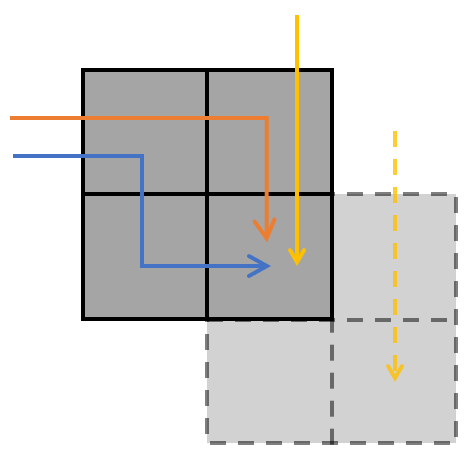
\includegraphics[scale = 0.5]{1.png}
        \end{center}
    \end{itemize}
\end{frame}

\begin{frame}{CF715D Create a Maze}
    \begin{itemize}
        \item 将若干个这种$2\times 2$的块拼在一起,每一次都会让之前的路径数量$\times 2$,同时我们又可以选择此时路径条数是否要加$1$
        \item 但是需要的块数是$\log T$级别的,而$n$只有$50$
        \item 如果我们将每一块最大能够表示出的路径数量调大,就可以降低需要的网格大小
    \end{itemize}
\end{frame}

\begin{frame}{CF715D Create a Maze}
    \begin{center}
        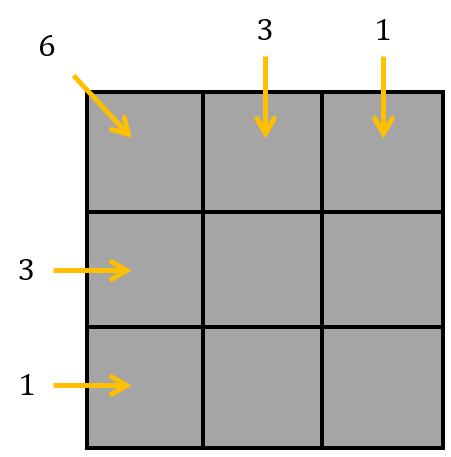
\includegraphics[scale = 0.5]{2.png}
    \end{center}
    \begin{itemize}
        \item 将每一块的大小调到$3$,那么一个块可以表示$6$条路径,也能表示$1\sim 5$的路径,对应$6$进制
        \item 需要的行数为$2 + 2\times \log_6T = 48$
    \end{itemize}
\end{frame}

\begin{frame}{CF715D Create a Maze}
    \begin{itemize}
        \item 在每个块外面需要构造出一条路径,以便接入这个块中
        \item 我们把第一行和第一列单独拿出来构造这样一条路径
    \end{itemize}
    \begin{center}
        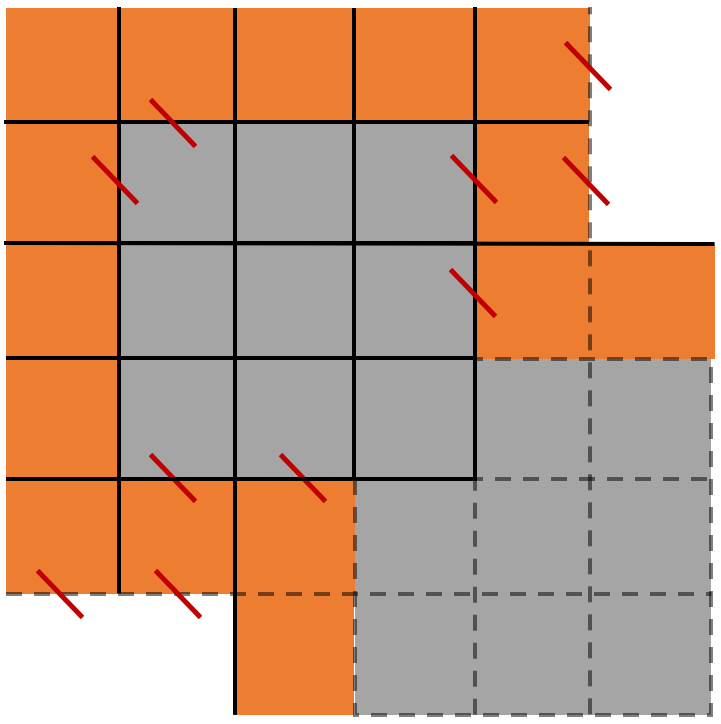
\includegraphics[scale = 0.4]{3.png}
    \end{center}
\end{frame}

\begin{frame}{CF794G Replace All}
    \begin{itemize}
        \item 给定两个仅包含$AB?$的字符串$X, Y$,其中$?$表示这个位置可以是$A$,也可以是$B$
        \item 你需要统计$01$串有序对$(S, T)$的数量,使得将$X, Y$中的$A$替换成$S$,$B$替换成$T$之后,$X, Y$相同,并且满足$|S|, |T|\leq n$且$S, T$均不能是空串
        \item 答案为所有可能$X, Y$串对应的$(S, T)$串的数量之和
        \item $|X|, |Y|, n\leq 3\times 10^5$,对$10^9 + 7$取模
    \end{itemize}
\end{frame}

\begin{frame}{CF794G Replace All}
    \begin{itemize}
        \item 我们首先考虑如果没有问号该怎么做
        \item 如果$X, Y$相同,那么显然他们起不到任何限制的作用,我们特判掉这种情况
        \item 定义两个字符串$s, t$互质当且仅当:
        \begin{itemize}
            \item $s = t$,或$t$与$s$互质
            \item $s$是$t$的前缀,且$s \bot t - s$
        \end{itemize}
        \item 类似于辗转相除法,可以发现两个字符串互质当且仅当他们存在公共周期
    \end{itemize}
\end{frame}

\begin{frame}{CF794G Replace All}
    \begin{block}{引理1}
        若$X, Y$不同,$S\bot T$是$(S, T)$合法的必要条件
    \end{block}
\end{frame}

\begin{frame}{CF794G Replace All}
    \begin{itemize}
        \item 我们找到$X, Y$的最长公共前缀,显然这个前缀无法起到任何限制作用
        \item 将这个前缀去掉,此时$X$的第一个字符与$Y$的第一个字符一定不同,一个是$A$,另一个是$B$
        \item 我们假设$|S|\leq |T|$
        \item 如果$X, Y$在被替换之后相同,那么此时$T$一定是$S$的前缀
        \item 将$T$改写为$S + x$,此时$X, Y$串中全部都是$S, x$两种串,这是原问题的一个子问题
        \item 这个递归的过程就是前面提到的辗转相除,因此$S\bot T$
    \end{itemize}
\end{frame}

\begin{frame}{CF794G Replace All}
    \begin{block}{引理2}
        $X, Y$所对应的$(S, T)$数量仅与$A, B$的数量有关,与排列方式无关
    \end{block}
\end{frame}

\begin{frame}{CF794G Replace All}
    \begin{itemize}
        \item $S\bot T$意味着$S, T$有公共周期,那么$S + T = T + S$
        \item 以$X$串为例,如果两个相邻的位置为$BA$,那么我们可以交换这两个位置使得最后得到的串不变
        \item 因此我们可以把$A$全部挪到前面去,把$B$全部堆到后面来
        \item 两个串的公共前缀以及公共后缀都是没有限制作用的,我们将他们去掉
        \item 此时一个串全是$A$,另一个串全是$B$
    \end{itemize}
\end{frame}

\begin{frame}{CF794G Replace All}
    \begin{itemize}
        \item 设$c_A$表示$A$的个数,$c_B$表示$B$的个数,接下来我们分类讨论
    \end{itemize}
    1. $c_A = 0, c_B = 0$
    \begin{itemize}
        \item 此时相当于要求$S \bot T$,方案数为
        $$\begin{aligned}
            \sum_{i = 1}^n \sum_{j = 1}^n 2^{\gcd(i, j)} &= \sum_{d = 1}^n 2^d \sum_{i = 1}^{\lfloor\frac nd\rfloor}\sum_{j = 1}^{\lfloor\frac nd\rfloor}[\gcd(i, j) = 1]\\
            &= \sum_{d = 1}^n 2^d \sum_{l = 1}^{\lfloor\frac nd\rfloor}\mu(l)\lfloor\frac n{dl}\rfloor^2\\
            &= \sum_{T = 1}^n \lfloor\frac nT\rfloor^2 \sum_{d\mid T} 2^d\mu(\frac Td)
        \end{aligned}$$
    \end{itemize}
\end{frame}

\begin{frame}{CF794G Replace All}
    2. $c_A = 0$或$c_B = 0$,且他们不同时为$0$
    \begin{itemize}
        \item 显然此时无解
    \end{itemize}
    3. $c_A\neq 0, c_B\neq 0$
    \begin{itemize}
        \item 我们将$c_A, c_B$同时除以它们的$\gcd$,不会影响答案
        \item 此时$c_A\bot c_B$,不妨设$c_A\leq c_B$
        \item 这意味着$S$有一个周期是$\frac{|S|}{c_B}$,且$|T| = |S|\times \frac{c_A}{c_B}$
        \item 因此,我们只需要确定$S$串,$T$串也随之确定了。$S$串一个周期的长度至多为$\lfloor\frac{n}{c_B}\rfloor$
        \item 方案数为$2^1 + 2^2 + \cdots + 2^{\lfloor\frac n{c_B}\rfloor} = 2^{\lfloor\frac n{c_B}\rfloor + 1} - 2$
    \end{itemize}
\end{frame}

\begin{frame}{CF794G Replace All}
    \begin{itemize}
        \item 现在考虑有问号的情况
        \item 假设抛开问号不管,$X$中$A$的数量减去$Y$中$A$的数量为$c_A'$,$B$同理。$X$中问号的数量为$a$,$Y$中问号的数量为$b$
        \item 假设在某一次给问号分配$A, B$的过程中,$X$中有$i$个问号为$A$,$Y$中有$j$个问号为$A$
        \item 此时我们可以得到
        $$\begin{aligned}
            c_A &= c_A' + i - j\\
            c_B &= c_B' + (a - i) - (b - j)\\
                &= c_B' + (a - b) - (i - j)
        \end{aligned}$$
        \item 容易发现它们的取值只与$i - j$有关,我们记此时的方案数为$f(i - j)$
    \end{itemize}
\end{frame}

\begin{frame}{CF794G Replace All}
    \begin{itemize}
        \item 枚举$X$中将多少个问号变成了$A$,$Y$中将多少个问号变成了$A$
        \item 那么答案就等于
        $$\begin{aligned}
            \sum_{i = 0}^{a} \sum_{j = 0}^{b} f(i - j){a\choose i}{b\choose j}
            &= \sum_{k = -b}^{a} f(k) \sum_{i = 0}^{a} {a\choose i}{b\choose i - k}\\
            &= \sum_{k = -b}^{a} f(k) \sum_{i = 0}^{a} {a\choose i}{b\choose b - i + k}\\
            &= \sum_{k = -b}^{a} f(k) {a + b\choose b + k}
        \end{aligned}$$
    \end{itemize}
\end{frame}

\begin{frame}{CF794G Replace All}
    \begin{itemize}
        \item 但是这样有个小问题
        \item 如果在确定问号是啥之后,$X,Y$两个串相同,此时我们是按照$c_A = 0, c_B = 0$,即$S\bot T$处理的,但是实际上此时$S, T$可以随便取
        \item 求出$X = Y$的方案数,从答案里面减去我们按照$c_A = 0, c_B = 0$计算的结果,再加上$\left(2^{n + 1} - 2\right)^2$即可
        \item 时间复杂度$O(n\log n)$
        \item \url{https://codeforces.com/contest/794/submission/71471572}
    \end{itemize}
\end{frame}

\end{document}